\documentclass[11pt]{article} % use larger type; default would be 10pt

\usepackage[utf8]{inputenc} % set input encoding (not needed with XeLaTeX)

\usepackage{tikz}
\usetikzlibrary{positioning}
\begin{document}

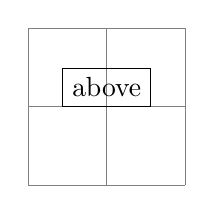
\begin{tikzpicture}
\draw[help lines] (0,0) grid (2,2);
%\node at (1,1) [above=2pt+3pt,draw] {above};
\node at (1,1) [above,draw] {above};
\end{tikzpicture}

\end{document}